\section{Intégration par lots et performances}\label{sec:perf}

\subsection{Vectorisation}

Dans un code EF, la loi est appelée sur tous les points de Gauss du maillage à chaque itération, et ces appels sont indépendants. La fonction écrite pour \emph{un} point se vectorise en une ligne :
\begin{lstlisting}
batched = jax.jit(jax.vmap(integrate, in_axes=(0, 0, None)))   # params partages
sigma, state = batched(eps[N,6], State(eps_p[N,6], p[N], alpha[N,6]), params)
\end{lstlisting}
Comme les deux branches de chaque \code{where} sont calculées, le coût d'un point ne dépend \emph{pas} de son état. Il n'y a ni divergence de branches sur GPU, ni masque vectoriel coûteux sur CPU. Dans nos données, 99,8\,\% des points plastifient, mais un lot entièrement élastique coûterait pareil. Le corollaire est qu'il est inutile d'espérer gagner du temps sur les points élastiques.

\subsection{Modèle de performance}

\begin{rappel}{modèle roofline}
Le temps d'un noyau est borné inférieurement par $\max\big(W/F,\ Q/B\big)$, où $W$ est le nombre d'opérations flottantes, $F$ le débit crête de calcul, $Q$ le volume de données échangé avec la mémoire et $B$ la bande passante~\cite{williams2009}. Le rapport $I=W/Q$ (flop/octet) est l'\emph{intensité arithmétique}. Si $I<F/B$ (le « point d'équilibre » de la machine), le noyau est limité par la mémoire, sinon par le calcul.
\end{rappel}

\paragraph{Comptage pour un point de Gauss.}
\begin{itemize}[nosep]
  \item \emph{Volume minimal} : lire $\eps,\epsp,p,\X$ (19 nombres) et écrire $\sig,\epsp,p,\X$ (19 nombres), soit $Q_{\min}=38$ mots, c'est-à-dire 304~octets en FP64 et 152 en FP32.
  \item \emph{Opérations} : XLA en compte 228 (\code{cost\_analysis}). En faisant varier le nombre d'itérations de Newton, on constate que ce compte n'inclut le corps de la boucle qu'une fois. L'estimation réelle est d'environ 300~flops et une dizaine d'exponentielles par point.
  \item \emph{Intensité} : $I\approx1$~flop/octet en FP64. C'est très faible : un CPU moderne a un point d'équilibre de 5 à 20~flop/octet. Le noyau est donc \textbf{limité par la mémoire} sur CPU.
\end{itemize}

\paragraph{Ce que fait réellement XLA.} L'examen du code compilé (\code{compiled.as\_text()}) montre que XLA ne produit pas \emph{un} noyau. Il en produit 12 fusions, plus une boucle \code{while} pour le Newton. Des intermédiaires de taille $N\times6$, comme $\bs\xi\tri$, sont donc écrits en mémoire puis relus par plusieurs consommateurs. Le trafic estimé par XLA est de 1072~octets par point en FP64, soit \textbf{3,5 fois le minimum}. Dérouler la boucle (\code{unroll=True}) ne change rien (1200~octets, débit identique à 5\,\% près). Pour atteindre le minimum il faudrait un noyau écrit à la main, par exemple en Pallas, Numba ou C++/CUDA, qui fasse tout en registres. C'est une piste d'optimisation identifiée, mais non réalisée ici.

\subsection{Mesures sur CPU}

Configuration : NumPy vectorisé et JAX CPU, FP64 et FP32, $N$ de $10^2$ à $3\times10^6$. On ne va pas jusqu'à $10^7$ : la version NumPy, avec ses temporaires, dépasse les 7~Go de la machine virtuelle. Chaque point de mesure est la médiane d'au moins 3 appels et d'au moins 0,3~s de mesure. La compilation est mesurée à part.

\begin{figure}[h]
\centering
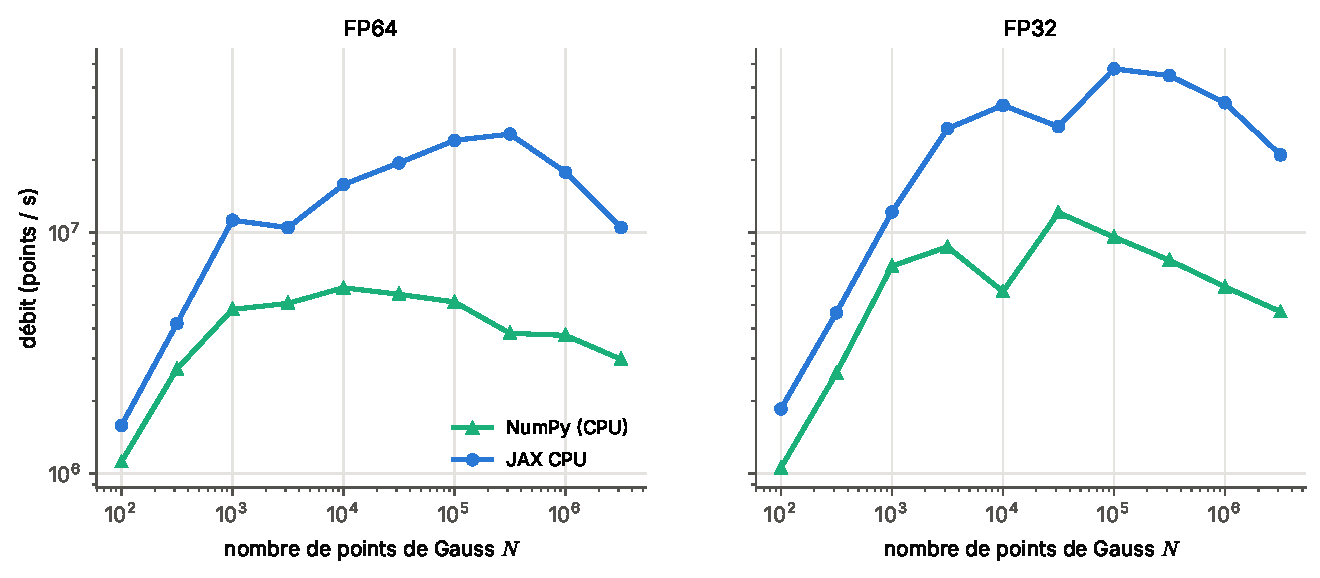
\includegraphics[width=\linewidth]{bench_cpu_throughput}
\caption{Débit (points de Gauss par seconde) en fonction de $N$, machine virtuelle 2 cœurs. Écrouissage Voce + Prager, 4 itérations de Newton local.}\label{fig:bench-thr}
\end{figure}

\begin{figure}[h]
\centering
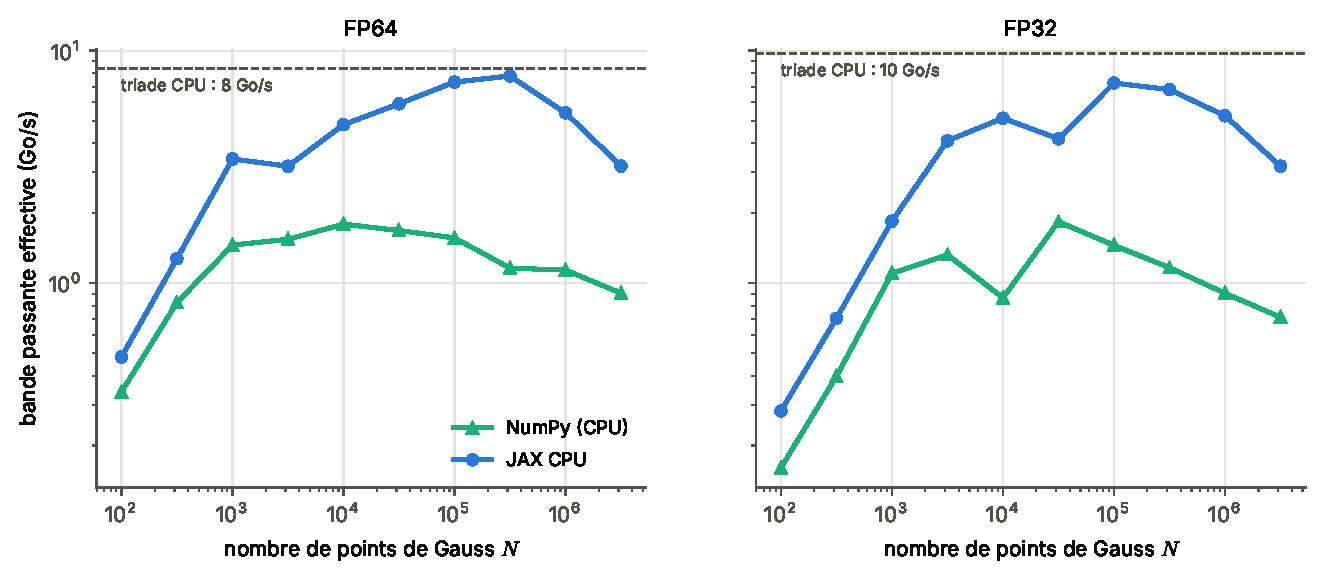
\includegraphics[width=\linewidth]{bench_cpu_bandwidth}
\caption{Bande passante effective calculée sur le volume \emph{minimal} (304~o/point en FP64), comparée à la bande passante d'une triade $z=ax+y$ sur de grands tableaux (mémoire principale).}\label{fig:bench-bw}
\end{figure}

\begin{table}[h]
\centering
\begin{tabular}{lcccc}
\toprule
 & \multicolumn{2}{c}{FP64} & \multicolumn{2}{c}{FP32}\\
\cmidrule(lr){2-3}\cmidrule(lr){4-5}
 & meilleur débit & à $N=3\times10^6$ & meilleur débit & à $N=3\times10^6$\\
\midrule
NumPy & $5{,}9\times10^6$ & $3{,}0\times10^6$ & $1{,}2\times10^7$ & $4{,}7\times10^6$\\
JAX CPU & $2{,}6\times10^7$ & $1{,}05\times10^7$ & $4{,}8\times10^7$ & $2{,}1\times10^7$\\
rapport JAX / NumPy & $4{,}3$ & $3{,}5$ & $4{,}0$ & $4{,}5$\\
\bottomrule
\end{tabular}
\caption{Débits mesurés (points/s). Temps de compilation JAX : 0,16 à 0,23~s, indépendant de $N$.}\label{tab:bench}
\end{table}

\paragraph{Lecture des résultats.}
\begin{enumerate}
  \item \textbf{Petits lots ($N\lesssim10^3$).} Le temps est dominé par le coût fixe d'un appel, environ 60~µs pour JAX : dispatch Python et lancement du noyau. Le débit croît alors linéairement avec $N$. Dans un code EF, cela plaide pour un appel par \emph{maillage} et non par élément.
  \item \textbf{Lots moyens ($10^4$ à $3\times10^5$).} Les données (30 à 100~Mo, auxquels s'ajoutent les intermédiaires) tiennent dans le grand cache L3 de la machine hôte (260~Mo). JAX atteint $2{,}6\times10^7$ points/s en FP64, soit 4,3 fois NumPy. Le gain vient de la fusion : NumPy matérialise chaque opération dans un temporaire de taille $N$, alors que XLA en élimine la plupart.
  \item \textbf{Grands lots ($N\ge10^6$).} Les données sortent du cache et le débit chute à $1{,}05\times10^7$ points/s. En volume \emph{réel} (1072~o/point), cela représente 11~Go/s, du même ordre que la bande passante de la triade (8,4~Go/s), une partie des intermédiaires restant en cache. Le noyau est donc bien limité par la mémoire. Le facteur 3,5 de trafic superflu se paie directement en temps.
  \item \textbf{FP32 contre FP64.} En FP32, le débit est 1,8 à 2 fois plus élevé, exactement le rapport des volumes de données. C'est une autre confirmation que le noyau est limité par la mémoire et non par le calcul.
  \item \textbf{Compilation.} 0,2~s par forme de tableau. C'est négligeable devant un calcul, mais \code{jit} recompile pour chaque nouveau $N$. Un code EF doit donc garder des formes fixes, en complétant les lots par du remplissage si nécessaire.
\end{enumerate}

\subsection{Mesures sur GPU : RTX~2050 portable}\label{sec:gpu}

\paragraph{Machine et méthode.} Portable Lenovo LOQ : processeur i5-12450HX (8 cœurs, 12 threads), carte NVIDIA GeForce RTX~2050 (architecture Ampere, 4~Go de GDDR6 sur un bus de 64~bits, PCIe~3.0~x8), pilote 595.99, JAX~0.12 avec CUDA~13. Les mesures sont faites avec le kit du dossier \code{gpu/} (annexe~\ref{app:repo}). Avant toute mesure, deux vérifications :
\begin{itemize}[nosep]
  \item les 77 tests passent sur la machine ;
  \item le GPU donne les mêmes contraintes que NumPy, avec un écart relatif de $1{,}1\times10^{-16}$ en FP64 et $1{,}3\times10^{-7}$ en FP32 (arrondi de la simple précision).
\end{itemize}

\paragraph{Les plafonds de la machine.} Le script \code{check\_gpu.py} mesure les limites matérielles qui servent de référence (tableau~\ref{tab:plafonds}).

\begin{table}[h]
\centering
\begin{tabular}{lcc}
\toprule
Grandeur & Mesurée & Théorique\\
\midrule
PCIe hôte $\to$ GPU & 4,9~Go/s & 7,9~Go/s\\
PCIe GPU $\to$ hôte & 2,2~Go/s & 7,9~Go/s\\
bande passante mémoire GPU (triade) & 91--94~Go/s & 112~Go/s\\
bande passante mémoire CPU (triade) & 20--21~Go/s & ---\\
calcul GPU FP32 (produit de matrices) & 5475~GFLOP/s & 6020~GFLOP/s\\
calcul GPU FP64 (produit de matrices) & 106~GFLOP/s & 94~GFLOP/s\\
rapport FP64 / FP32 & 1/52 & 1/64\\
latence d'un appel JAX & 31~µs & ---\\
\bottomrule
\end{tabular}
\caption{Plafonds mesurés sur la machine.}\label{tab:plafonds}
\end{table}

\begin{piege}{le FP64 sur GPU grand public}
Une carte « gaming » n'a qu'une unité FP64 pour 64 unités FP32. Les cartes de calcul (A100, H100) ont un rapport de 1/2. La mesure confirme l'ordre de grandeur : 106~GFLOP/s en FP64 contre 5475 en FP32, soit un rapport de 1/52. En FP64, la RTX~2050 calcule donc moins vite que le processeur du même portable.
\end{piege}

\begin{figure}[h]
\centering
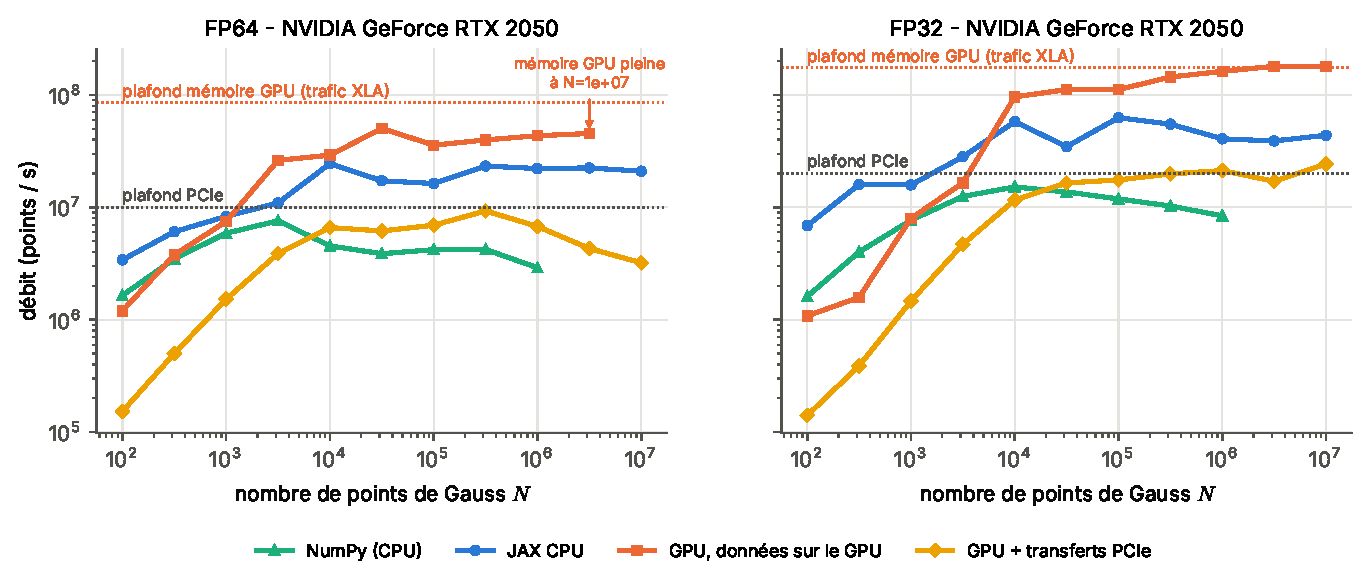
\includegraphics[width=\linewidth]{gpu_throughput_izanami-LOQ-15IAX9}
\caption{Débit mesuré en fonction de $N$ sur la machine équipée de la RTX~2050. Les pointillés sont les plafonds calculés à partir des mesures du tableau~\ref{tab:plafonds}. Plafond mémoire GPU : triade divisée par le trafic réel d'XLA (1072~o/point en FP64, 536 en FP32). Plafond PCIe : envoi de 19 nombres et retour de 19 nombres par point, aux débits mesurés.}\label{fig:gpu-thr}
\end{figure}

\begin{figure}[h]
\centering
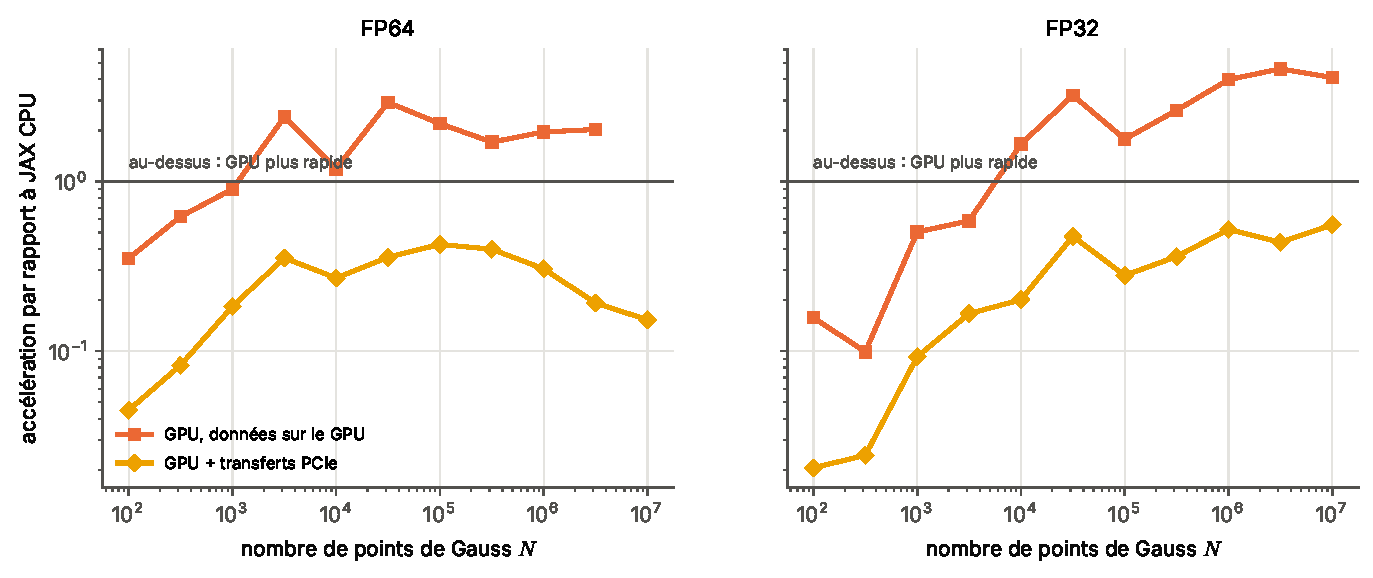
\includegraphics[width=\linewidth]{gpu_speedup_izanami-LOQ-15IAX9}
\caption{Accélération par rapport à JAX CPU (12 threads). Au-dessus de 1, le GPU est plus rapide.}\label{fig:gpu-speedup}
\end{figure}

\begin{table}[h]
\centering
\begin{tabular}{lcccc}
\toprule
 & NumPy & JAX CPU & GPU, données résidentes & GPU + transferts\\
\midrule
FP64 & $2{,}9\times10^6$ & $2{,}2\times10^7$ & $4{,}3\times10^7$ ($\times2{,}0$) & $6{,}8\times10^6$ ($\times0{,}31$)\\
FP32 & $8{,}4\times10^6$ & $4{,}1\times10^7$ & $1{,}6\times10^8$ ($\times4{,}0$) & $2{,}1\times10^7$ ($\times0{,}52$)\\
\bottomrule
\end{tabular}
\caption{Débits mesurés (points/s) à $N=10^6$. Entre parenthèses : l'accélération par rapport à JAX CPU.}\label{tab:gpu}
\end{table}

\paragraph{Lecture des résultats.}
\begin{enumerate}
  \item \textbf{Les plafonds se vérifient presque au point près.}
  \begin{itemize}[nosep]
    \item En FP32, le GPU avec données résidentes atteint $1{,}79\times10^8$ points/s pour un plafond mémoire de $1{,}76\times10^8$ : il est exactement \textbf{limité par la bande passante}, avec le trafic réel d'XLA (3,5 fois le minimum, section~\ref{sec:perf}).
    \item Sur CPU, JAX en FP64 atteint $2{,}2\times10^7$ points/s pour un plafond de $21{,}4\ \text{Go/s} / 1072\ \text{o} = 2{,}0\times10^7$ : également limité par la mémoire.
    \item La découpe du noyau en 12 fusions par XLA coûte donc le même facteur 3,5 sur CPU et sur GPU.
  \end{itemize}
  \item \textbf{En FP64, le GPU est limité par ses unités de calcul.} Il plafonne à $4{,}5\times10^7$ points/s, soit seulement 53\,\% de son plafond mémoire. La division, la racine carrée et l'exponentielle de Voce en FP64 coûtent chacune des dizaines d'opérations sur des unités 52 fois moins nombreuses. C'est pourquoi le rapport FP32/FP64 sur GPU vaut 4 : ce n'est ni 2 (rapport des volumes de données, comme sur CPU), ni 52 (rapport des unités de calcul).
  \item \textbf{Avec données résidentes, le GPU gagne}, d'un facteur 2 en FP64 et de 4 à 4,6 en FP32 pour les grands lots. Le point de bascule est à $N\approx3\times10^3$ en FP64 et $10^4$ en FP32. En dessous de $10^3$ points, le GPU est plus lent : le coût fixe d'un lancement (31~µs pour un appel vide, environ 80~µs pour le noyau) domine.
  \item \textbf{Avec les transferts, le GPU perd toujours.} Il atteint au mieux 0,43 fois la vitesse du CPU en FP64 et 0,56 fois en FP32. Le plafond PCIe calculé avec les débits mesurés,
  \[
  \Big(\tfrac{152\ \text{o}}{4{,}86\ \text{Go/s}}+\tfrac{152\ \text{o}}{2{,}20\ \text{Go/s}}\Big)^{-1} = 1{,}0\times10^7\ \text{points/s en FP64},
  \]
  est atteint à 93\,\% ($9{,}3\times10^6$). Il reste inférieur au débit du CPU seul ($2{,}2\times10^7$).
  \item \textbf{Où passe le temps} (figure~\ref{fig:gpu-bd}) : à $N=10^7$, le calcul ne représente que 11 à 13\,\% du temps. Le retour des résultats en prend 51 à 64\,\% et l'envoi 25 à 36\,\%. Le retour est plus lent que l'envoi parce que la mémoire de l'hôte n'est pas « verrouillée » (\emph{pageable}) : le pilote doit faire une copie intermédiaire.
  \item \textbf{La mémoire de 4~Go limite la taille des lots.} À $N=10^7$ en FP64, la version « données résidentes » échoue : XLA demande 3,04~Go d'arguments pour une limite de 2,97~Go. La version avec transferts fonctionne grâce au découpage en blocs de $2^{20}$ points.
\end{enumerate}

\begin{figure}[h]
\centering
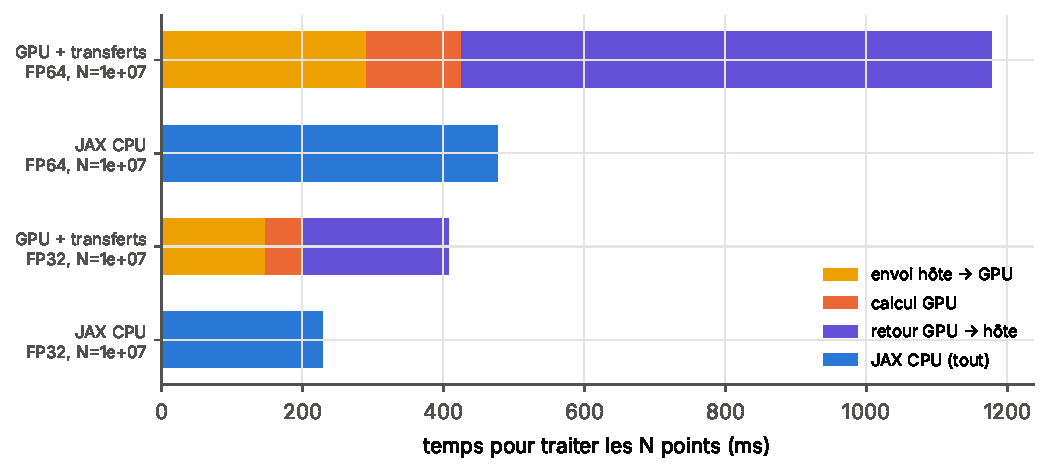
\includegraphics[width=0.85\linewidth]{gpu_breakdown_izanami-LOQ-15IAX9}
\caption{Décomposition du temps à $N=10^7$ : envoi, calcul et retour (chaque étape synchronisée), comparés au temps total de JAX CPU.}\label{fig:gpu-bd}
\end{figure}

\paragraph{Une limite de la mesure.} Aux plus grands $N$ en FP64, le débit de bout en bout avec transferts chute ($3{,}2\times10^6$ points/s à $N=10^7$). Pourtant, la somme des trois étapes mesurées séparément ne fait que 1,18~s, contre 3,1~s de bout en bout. L'écart vient d'un coût côté hôte : les 1,5~Go de tableaux de sortie étaient alloués à chaque répétition, et le système doit fournir ces pages mémoire au premier accès. Le kit a été corrigé pour allouer les sorties une seule fois. Même avec la somme des étapes ($8{,}5\times10^6$ points/s), le GPU reste 2,5 fois plus lent que le CPU : la conclusion ne change pas.

\paragraph{Comparaison avec le modèle a priori.} Avant de disposer de la machine, un modèle roofline avait été construit à partir des caractéristiques constructeur (tableau~\ref{tab:modele}).

\begin{table}[h]
\centering
\small
\begin{tabular}{lcc}
\toprule
Quantité & Prédiction & Mesure\\
\midrule
GPU résident, FP32 & $1{,}7$ à $5{,}9\times10^8$ & $1{,}8\times10^8$ (= borne XLA)\\
GPU résident, FP64 & $0{,}8$ à $1{,}9\times10^8$ & $4{,}5\times10^7$\\
GPU + transferts, FP64 & $\le2\times10^7$ (6~Go/s) & $9{,}3\times10^6$ (retour 2,2~Go/s)\\
GPU rentable avec transferts ? & non & non\\
\bottomrule
\end{tabular}
\caption{Modèle a priori contre mesures (points/s).}\label{tab:modele}
\end{table}

Le modèle avait raison sur la conclusion principale, et sur le FP32. Il était trop optimiste de 2 à 4 en FP64, car il sous-estimait le coût des fonctions spéciales en double précision sur ces unités. Il était aussi trop optimiste d'un facteur 2 sur le PCIe, car le retour vers l'hôte est deux fois plus lent que l'envoi.

\subsection{Conséquences pour une interface code\_aster--JAXMat}

\begin{itemize}
  \item \textbf{Transférer tout l'état à chaque appel n'est pas rentable}, quel que soit $N$. Les mesures le confirment.
  \item \textbf{Garder les variables internes sur le GPU} entre les itérations de Newton change la donne. L'état ($\epsp$, $p$, $\X$) ne voyage plus : seuls $\eps$ (6 nombres) et $\sig$ (6 nombres) circulent, soit 96~o/point en FP64 au lieu de 304. Le plafond PCIe passe alors à $3{,}2\times10^7$ points/s, au-dessus du CPU ($2{,}2\times10^7$). C'est l'expérience à faire en priorité.
  \item \textbf{La tangente ne doit pas revenir sur le CPU.} Avec 36 nombres de plus par point, le plafond PCIe retombe à $6\times10^6$ points/s. Pour profiter du GPU avec un Newton complet, l'assemblage de $\mathbf{K}$ doit lui aussi se faire sur le GPU.
  \item \textbf{La mémoire hôte verrouillée} (\code{memory\_kind="pinned\_host"} dans JAX) devrait rapprocher le retour des 6 à 7~Go/s du bus PCIe.
  \item \textbf{FP32 ou précision mixte ?} Le gain du FP32 sur GPU (facteur 4) est tentant, mais une tangente en simple précision limite la précision de la convergence de Newton (section~\ref{sec:maths}). Une piste est la précision mixte : la loi en FP32, le résidu d'équilibre en FP64.
\end{itemize}

\subsection{Reproduire les mesures}\label{sec:protocole-gpu}

Le dossier \code{gpu/} contient un kit autonome, documenté dans \code{gpu/README\_GPU.md} :
\begin{lstlisting}[language=bash]
bash gpu/setup_gpu.sh            # venv + jax[cuda12/13] selon le pilote (une fois)
source .venv-gpu/bin/activate
bash gpu/run_all.sh              # tests, diagnostic, benchmark, figures, archive
\end{lstlisting}
Le benchmark vérifie d'abord l'exactitude du GPU contre NumPy. Il traite les grands lots par blocs de taille fixe, pour éviter de manquer de mémoire et de recompiler, et mesure séparément l'envoi, le calcul et le retour. Il désactive aussi la pré-allocation de JAX (\code{XLA\_PYTHON\_CLIENT\_PREALLOCATE=false}).
